\documentclass{BachelorBUI}

\usepackage[utf8]{inputenc}
\RequirePackage[babel,english=american]{csquotes} %% context sensitive quotations
\raggedbottom
\lstset{
 language={Matlab},
}
\sisetup{output-decimal-marker = {,},
range-phrase = --,
group-separator = {~},
per-mode = symbol,
list-final-separator={ and }}

%----------------------------------------------------------------------------------------
% Graphics
%----------------------------------------------------------------------------------------
\graphicspath{{images/}}

%----------------------------------------------------------------------------------------
% New commands
%----------------------------------------------------------------------------------------
\newcommand{\eg}{\mbox{e.\,g.}\xspace}
\newcommand{\Name}[1]{\textsc{#1}}

%----------------------------------------------------------------------------------------
% Acronyms
%----------------------------------------------------------------------------------------
\usepackage{acro}
\acsetup{list/display=used}
\input{acronyms}

%----------------------------------------------------------------------------------------
% Settings of document structure depth
%----------------------------------------------------------------------------------------
\setcounter{secnumdepth}{3}
\setcounter{tocdepth}{3} 

%----------------------------------------------------------------------------------------
% Title and author information
%----------------------------------------------------------------------------------------
\usepackage[style=authoryear,backend=biber,maxcitenames=2]{biblatex}
\ExecuteBibliographyOptions{%
 giveninits=true, maxbibnames=99}%
\DefineBibliographyStrings{english}{%
andothers={et\;al\adddot},
urlseen = {Accessed on}
}
\addbibresource{references.bib}
\setcounter{biburllcpenalty}{9000}% Lowercase
\setcounter{biburlucpenalty}{9000}% Uppercase

%----------------------------------------------------------------------------------------
% Title and author information
%----------------------------------------------------------------------------------------
\title{Plant Disease Classification:\\[0.5em]\LARGE An Approach using Convolutional Neural Networks}
\authorname{Jakub Dunaj} 
\email{e12121285@student.tuwien.ac.at} 
\MatrNr{12121285} 
\thesislanguage{en-US} 
\keywords{bachelor's thesis\sep plant disease classification\sep convolutional neural networks\sep CNNs\sep}

%----------------------------------------------------------------------------------------
% Begin of the document
%----------------------------------------------------------------------------------------
\begin{document}
\selectlanguage{english}
\begin{filecontents}[overwrite]{\jobname.xmpdata}
\makeatletter
\Title{\@title}
\Author{\@authorname}
\Language{\@thesislanguage}
\Keywords{\@keywords}
\Publisher{TU Wien}
\makeatother
\end{filecontents}

%----------------------------------------------------------------------------------------
% Title
%----------------------------------------------------------------------------------------
\maketitle

%----------------------------------------------------------------------------------------
% Abstract
%----------------------------------------------------------------------------------------
\begin{abstract}
\end{abstract}

%----------------------------------------------------------------------------------------
% Table of contents
%----------------------------------------------------------------------------------------
\clearpage
\tableofcontents

%----------------------------------------------------------------------------------------
% Bachelor's thesis
%----------------------------------------------------------------------------------------
\clearpage
\section{Introduction}

\section{Thesis Focus and Related Work}

    \subsection{Machine Learning: An Overview}
    \label{sec:machine-learning-overveiw}

        I want the reader of my thesis to think about a random sequence of characters 'd' and 'f'. The reader can try to write down a random sequence of maybe 10 to 20 of these two characters. How random does the reader think the sequence is? Are there any patterns present in the sequence? In fact, this is hard to tell only from one short sequence. What about thousand sequences or one very long sequence? Does the reader think that those would be random and unique even if she or he tried very hard? I would advise the reader to have a look at the following website \url{https://people.ischool.berkeley.edu/~nick/aaronson-oracle/index.html} and try the website out. The algorithm on the website attempts to predict whether the next typed character will be 'd' or 'f'. The algorithm predicts the next typed character based on the sequence of 'd's and 'f's the user has typed so far. In figure \ref{fig:website-predicting-typed-characters}, the algorithm could predict my next typed character with a probability of 67\%. 

        \begin{figure}[h]
            \centering
            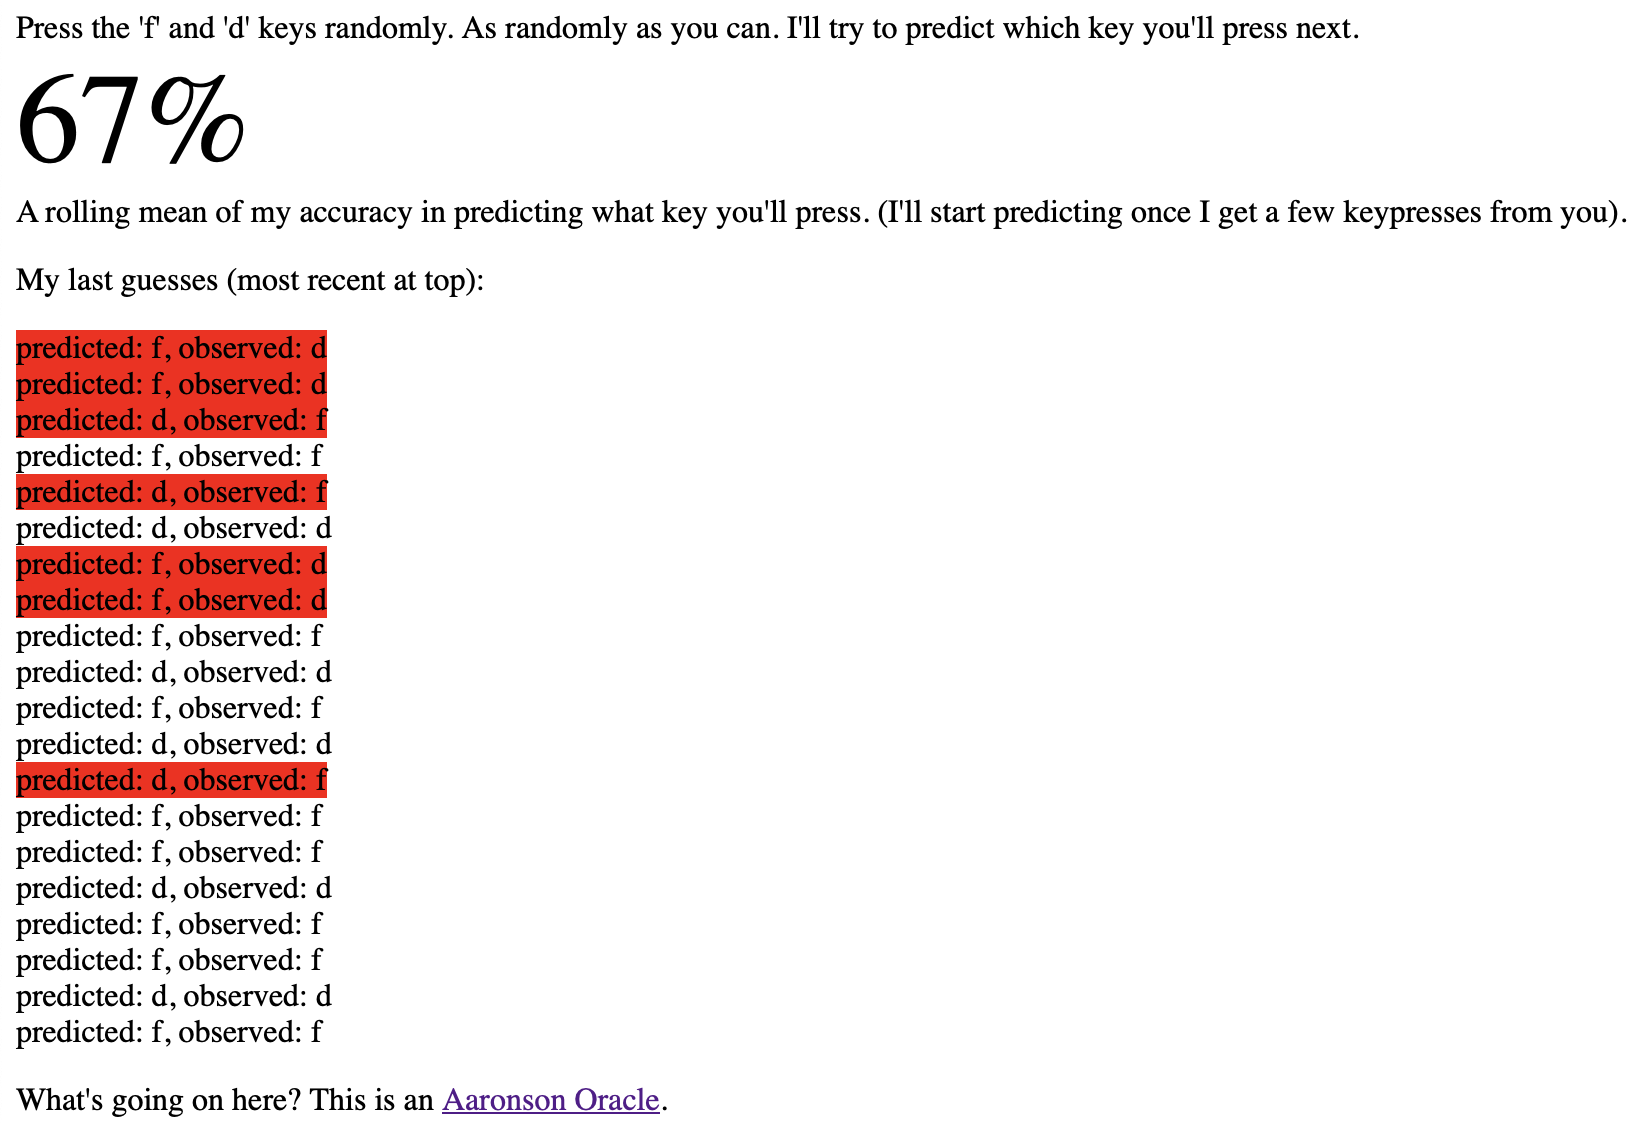
\includegraphics[width=0.8\textwidth]{website_predicting_typed_characters.png}
            \caption{Website predicting whether the user will type 'd' or 'f' next (\cite{Aaronson_Oracle:2024})}
            \label{fig:website-predicting-typed-characters}
        \end{figure}

        The website is based on the book "Quantum Computing since Democritus" by Scott Aaronson. \textcite{Aaronson:2013} wrote a simple program predicting whether the next typed character would be 'd' or 'f'. The author found that the algorithm was successful 70\% of the time. To answer the rhetorical questions asked at the beginning of this sections, humans can't generate truly random sequences of 'd's and 'f's. There is something fundamental in our sequences making the next character predictable. That is true for all human-generated data. In fact, we leave patterns in all our data. This is tightly coupled with human behavior and the complexity of our everyday tasks. Humans don't behave randomly. We exercise different behavioral patters instead. We can observe this phenomenon all around us. For example, fashion trends differ between generations or age groups. Young people wear different styles of clothes than elderly people. People with higher income spend their money differently than people with lower income. Sporty people are maybe more health conscious and tend to buy healthier groceries than general population. 
        
        We can think, for example, of a large fashion retailer offering thousands of articles in thousands of physical stores and through a website. This retailer wants to know which products or styles and when are popular among customer. The retailer stores different data from every transaction made online or in-store by customers enrolled in the bonus program: customer gender, customer age, articles bought, total price, store location, current weather, current clothing season, and many others. Customers don't buy their clothes randomly. They are influenced by many different factors, such as their gender or age group. From this huge amount of collected data, the retailer could infer different behavioral patterns and accordingly modify its offer to maximize profits. The retailer could ask the following question: "What products do 35-year-old customers buy in Vienna during the summer after 2PM?". Clearly, there is no standard algorithm for this complex multidimensional problem. We don't have the knowledge about the behavioral patterns of the customers. Instead, we need to create a mechanism that would infer these patterns in customers' buying habits from the transaction data. That is where the machine learning comes into play. It allows us to predict possible outputs based on a specific input of parameters. In the specified problem, the input parameters would be the customer's age, store location, clothing season and purchase time. We would expect the mechanism to predict the customers' preferences from these input parameters. The mechanism would obtain and infer the knowledge from the transaction data.

        More formally, we can define machine learning as creating and applying computational methods using data to make accurate predictions or optimize different complex tasks (\cite{Mohri:2018}). These computational methods consist of learning algorithms processing the training data and models representing the knowledge gained from the learning process (\cite{Alpaydin:2014}). A model is defined by a set of parameters influencing model's response to a given input (\cite{Alpaydin:2014}). A model can be, for example, simple linear function or a complex model such as a neural network. During the learning process, the learning algorithm optimizes model's parameters using the training data (\cite{Alpaydin:2014}). The final trained model approximates the patterns and regularities present in the data and provides useful representation of the knowledge gained during the training process (\cite{Alpaydin:2014}). We can refer to the training data as the experience the training algorithms use to train machine learning models. A trained model may not contain all information present in the training data, but it makes predictions that are accurate enough and thus useful (\cite{Alpaydin:2014}). From the computer science perspective, there are different aspects of machine learning that have to be considered (\cite{Alpaydin:2014}). The learning algorithm must efficiently solve the optimization problem of model's parameters. There must be an efficient way to store and process large amounts of training data, and the model's algorithmic representation must be efficient as well.
        
        Machine learning is a subfield of artificial intelligence. To be and behave intelligent, a machine learning model has to have the ability to learn and adapt to the changes in the training data (\cite{Alpaydin:2014}). The changes in the training data result from the changes in the experience the data describes. The model has to adapt to these changes through learning to accurately approximate the experience. Furthermore, because of the ability of the machine learning models to learn and adapt, there is no need to program the model explicitly (\cite{Alpaydin:2014}). The trained model may be predictive, descriptive, or have both of the features at the same time (\cite{Alpaydin:2014}). This means that the model can make predictions about the future or describe the knowledge from the data, or even do both. All the model's knowledge is inferred from the training data.

        The prediction accuracy of a model depends on the size of training data and the model complexity (\cite{Murphy:2022}). A model is accurate when it can generalize well (\cite{Mohri:2018}). Generalization means that the model makes accurate predictions not only about the training data but also about unseen data (\cite{Bishop:2006}). To achieve good model generalization, a trade-off between the size of the training data and the model complexity must be done (\cite{Bishop:2006,Mohri:2018}). The model complexity can be defined as the number of parameters of the model (\cite{Bishop:2006}). When the training data is small and the model is too complex, it may generalize poorly to unseen data (\cite{Mohri:2018}). This is known as overfitting of the trained model (\cite{Mohri:2018}). On the other hand, a model that is too simple may not be able to achieve sufficient accuracy on the training data. This is known as underfitting (\cite{Mohri:2018}). 

        What kind of problems can be solved using machine learning? When do we use machine learning instead of explicitly programming a computer program? There are two aspects of the problems we have to consider. These are the complexity of the problem and the need for adaptivity of the computer program (\cite{Shalev-Shwart:2014}). Complex problems may require mimicking animal or human intelligence or even go beyond human capabilities (\cite{Shalev-Shwart:2014}). The adaptivity of the computer program is its ability to learn from a changing experience without explicit programming (\cite{Shalev-Shwart:2014}). Machine learning is used in a variety of problem settings that involve: natural language processing, speech processing, computer vision, computational biology, and many others (\cite{Mohri:2018}).

        Further, I want to discuss machine learning approaches and neural networks as a machine learning model to give more insights into machine learning. % maybe adding here some other machine learning models -> Support Vector Machines (SVM), K-nearest Neighbors (KNN), Decision Trees, Random Forest, K-means Clustering

        \subsubsection{Machine Learning Approaches}
        \label{sec:machine-learning-approaches}

            Machine learning approaches can be divided into different categories based on the type of experience machine learning algorithms use to train machine learning models (\cite{Goodfellow:2016}). The different categories of machine learning approaches are: supervised, unsupervised and reinforcement learning. These categories are groups of machine learning algorithm that use the same type of experience for the training of models. As mentioned in the previous sections, the experience is the training data used by a machine learning algorithm. Each of these categories of machine learning algorithms can be applied to different groups of learning problems. Next, I want to discuss the different categories of machine learning algorithms and also the groups of learning problems the categories of algorithms are used for.
    
            \paragraph{Supervised Learning}
            \label{para:supervised-learning}
                
                In supervised learning, the objective is to train a machine learning model using labeled training data to map an input to a correct output (\cite{Alpaydin:2014}). This learning approach is called supervised because the training data consists of input--output pairs (\cite{Murphy:2022}). This means that the output is known for every input. The input of a machine learning algorithm is called a feature, which is typically a fixed-dimensional vector of numbers (\cite{Murphy:2022}). The output of a trained model is typically also a fixed-dimensional vector (\cite{Bishop:2006}). A machine learning algorithm uses the input vector from the problem instance to train a model that maps this input to an output vector (\cite{Bishop:2006}). An output that is associated with an input is also known as a label (\cite{Murphy:2022}). During a supervised learning process of a machine learning model, a machine learning algorithm tries to minimize the approximation error between the true label and the label predicted by the trained model (\cite{Alpaydin:2014}). A machine learning algorithm does this by adjusting the parameters of the trained model (\cite{Alpaydin:2014}). A feature used by a machine learning algorithm could be a vector of values representing pixels of an image (\cite{Murphy:2022}). The label of such an input vector could be the name of an object that is represented in the image. 

                There are two different groups of machine learning problems that can be solved using a supervised learning approach: classification and regression problems. In classification problems, every problem instance belongs to a class. The task in classification problems is the prediction of the class of a problem instance (\cite{Goodfellow:2016}). In supervised learning, the problem instance and its associated class build the input--output pair. The output of a machine learning model trained to solve a classification problem is typically a probability distribution over all classes occurring in the problem setting (\cite{Goodfellow:2016}). Classification problems could be simple binary classification problems or problems involving many different discrete classes. There are different examples of classification problems: pattern recognition, face recognition, medical diagnosis, speech recognition, natural language processing, biometrics, knowledge extraction, outlier detection, or for example novelty extraction (\cite{Alpaydin:2014}). For example, a medical diagnosis problem would be predicting a disease based on a patient's medical status. The input vector could contain the patient's age, gender, current health issues, or past medical history. The machine learning model would then predict the disease based on this information.

                Regression problems are problems of predicting one or more continuous variables for a problem instance (\cite{Bishop:2006}). An example of a regression problem would be the price prediction for a used car (\cite{Alpaydin:2014}). The input vector could contain the car's brand, year, mileage, fuel consumption, or color. The label of this input would then be the price for the specific car. The input--output pairs in training data would consist of car features and prices. Another regression problem would be the prediction of company stock prices based on different markers describing the company's performance (\cite{Mohri:2018}).

            \paragraph{Unsupervised Learning}
            \label{para:unsupervised-learning}

                Supervised machine learning algorithms use labeled training data to create a machine learning models that map the inputs  to learned outputs. In unsupervised learning, the training data consists only of fixed-dimensional input vectors without any labels (\cite{Bishop:2006}). The objective of unsupervised learning is to find regularities in the training data (\cite{Alpaydin:2014}). The machine learning algorithms use only the input vectors from the unlabeled training data to train a machine learning model that is able to find regularities or structures in the input space (\cite{Alpaydin:2014}). 
                There are three different groups of problems that can be solved applying supervised learning algorithms: clustering, density estimation and dimensionality reduction problems for visualization. 
                
                There are various groups of machine learning problems that can be solved using an unsupervised machine learning approach. The partitioning of problem instances into homogeneous subsets is called clustering (\cite{Mohri:2018}). An example of a clustering problem is image compression (\cite{Alpaydin:2014}). A machine learning algorithm would search for clusters of pixels with similar colors. The average pixel color for the pixel regions is then computed. Saving information only about the location of the pixel regions and about the average color of the regions compresses the size of an image. Another group of problems is the dimensionality reduction problems (\cite{Mohri:2018}). If the problem instances have a large number of parameters, the input vectors are of high dimension, there is often a need to search for lower-dimensional representation of problem instances (\cite{Mohri:2018}). The high dimensionality of input vectors is reduced to speed up computations done on the data or to extract only parameters of problem instances that are useful and significant (\cite{Mohri:2018}). 

            \paragraph{Reinforcement Learning}
            \label{para:reinforcement-learning}

                In reinforcement learning, a learning algorithm tries to find a solution, sequence of actions, to a problem by interacting with the environment (\cite{Alpaydin:2014}). In contrast to supervised or unsupervised learning algorithms, a reinforcement learning algorithm does not have any prepared training data to use to find the best sequence of actions (\cite{Mohri:2018}). Instead, the learning algorithm, also called learner or agent, collects the data by exploring an environment using the trial and error process (\cite{Bishop:2006}). When interacting with the environment, the agent receives rewards or penalties for its actions (\cite{Alpaydin:2014}). Based on the rewards or penalties, the learner tries to modify its future actions to maximize the reward (\cite{Mohri:2018}). By maximizing the reward, the learner searches for the optimal solution to a given problem (\cite{Bishop:2006}). The resulting sequence of actions leading to the optimal solution is also called a policy. The reward or penalty that the learner receives is only for its immediate action (\cite{Mohri:2018}). That is why the learner has to also learn from its past actions to assess how its future actions will alter the goodness of the policy (\cite{Alpaydin:2014}). This is also called the exploration versus exploitation dilemma (\cite{Alpaydin:2014}). The learner has to decide between exploring the environment to gain more information and exploiting the information it already has collected (\cite{Alpaydin:2014}). An example of a problem that can be solved by a reinforcement learning algorithm is teaching a learner to play chess (\cite{Alpaydin:2014}). There are about $10^{120}$ different possible chess games (\cite{Shannon:1988}). It is computationally infeasible to use supervised or unsupervised learning approach and list all of the possible piece positions or games. In reinforcement learning setting, one move done by the learner leaning to play chess in insignificant on itself. The learner receives the feedback after completing the whole game. Receiving reward or penalty depends on winning or losing a game. This means that the learner learns the goodness of the complete sequence of moves.

        \subsubsection{Neural Networks}
    \subsection{Deep Learning: A Subset of Machine Learning}
        \subsubsection{Deep Neural Networks}
        \subsubsection{Convolutional Neural Networks (CNNs)}
            \paragraph{CNN Architecture}
                \subparagraph{Convolutional Layer}
                \subparagraph{Pooling Layer}
                \subparagraph{Fully Connected Layer}
            \paragraph{Common CNN Architectures in Plant Disease Classification}
                \subparagraph{AlexNet}
            \paragraph{Transfer Learning}
            \paragraph{Key Technologies in CNN Development}
        \subsubsection{Deep Learning: Impact on Agriculture}
    \subsection{Recent Advancements in Plant Disease Classification}

\section{Design}
    \subsection{Models of CNNs for Plant Disease Classification}
        \subsubsection{Architecture of CNN Model}
        \subsubsection{Dataset}
        \subsubsection{Training and Validation}
        \subsubsection{Model Evaluation}
    \subsection{Web-based Application}
        \subsubsection{Frontend Design}
        \subsubsection{Backend Design}
        
\section{Development}
    \subsection{CNN Model Training and Validation}
    \subsection{Web-based Application Development}
        \subsubsection{Frontend Development}
        \subsubsection{Backend Development}

\section{Web-based Application Walkthrough}

\section{Discussion}

\section{Conclusion}

%----------------------------------------------------------------------------------------
% References
%----------------------------------------------------------------------------------------
\clearpage
\printbibliography

\end{document}